\documentclass{beamer}
\usepackage{ctex} %注意这个宏包
\usepackage{color}
\usepackage{graphics,graphicx}
\usepackage{pstricks,pst-node,pst-tree}
\usetheme{Boadilla}
\usecolortheme{beaver}
\usepackage{pstricks}
\usepackage{pst-plot}
\CTEXoptions[today=old]
\setCJKmainfont[BoldFont={SimHei},ItalicFont={KaiTi}] {WenQuanYi Micro Hei Mono}
\title{MapReduce\\ Simplified Data Processing on Large Clusters}
\author{严春伟}
\institute[PKUSZ]{
    互联网研发中心\\
}
\date{\today}

\begin{document}
% ------------- title page ----------------------------
%--- the titlepage frame -------------------------%
\begin{frame}
  \titlepage
\end{frame}

\section{Begin}
\begin{frame}
\frametitle{Outline}
\tableofcontents
\end{frame}

\section{Introduction}
\begin{frame}
\frametitle{Motivation}
    \begin{block}{大数据的处理}
        \begin{enumerate}
            \item Google至少有$8*10^9$个网页
            \pause
            \item 成效和成本
            \pause
            \item 利用成百上千的CPU
        \end{enumerate}
    \end{block}
    \begin{block}{MapReduce的解决方案}
        \begin{enumerate}
        \item 自动化的并行分发控制
        \item 容错性
        \item I/O调度
        \end{enumerate}
    \end{block}
\end{frame}

\begin{frame}
    \frametitle{What is Map/Reduce}
    \begin{block}{Map in LISP(Scheme)}
        \begin{itemize}
        \item (\textbf{map} f list$\left[list_1, list_2, \cdots, list_n \right]$)
        \item (\textbf{map} square (list 1 2 3 4))
            \begin{itemize}
            \item (1 4 9 16)    
            \end{itemize}
        \end{itemize}
    \end{block}
    
    \begin{block}{Reduce in LISP}
        \begin{itemize}
        \item (\textbf{reduce} f list$\left[list_1, list_2, \cdots, list_n \right]$)
        \item (\textbf{reduce} + 0 (list 1 4 9 16))
            \begin{itemize}
            \item (+ 16 (+ 9 (+ 4 (+ 1 0))))
            \item 30
            \end{itemize}
        \end{itemize}
    \end{block}
\end{frame}

\section{编程模型}
\begin{frame}{Key/Value}
    \begin{itemize}
    \item (\textbf{map} mapper list$\left[(key,val)_1, (key,val)_2, \cdots, (key,val)_n \right]$)
        \begin{itemize}
        \item map对list中每一个(key,val)键值处理
        \item list$\left[(key,(mapper \quad val))_1, (key,(mapper \quad val))_2, \cdots\right]$ 
        \end{itemize}
    \item reduce(key, vals)
        \begin{itemize}
        \item 对每一个独特的key合并val
        \item 最终的输出
        \end{itemize}
    \end{itemize}
\end{frame}

%-- illustrator --
\begin{frame}[c]{Count Words in Docs}
    \begin{block}{Algorithm Code Demo}
    \begin{center}
    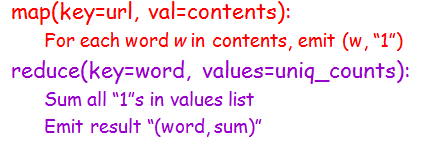
\includegraphics[height=60pt]{keyan/map1.png}
    \end{center}
    \end{block}

    \begin{block}{Count, Illustrated}
    \begin{center}
    
\includegraphics[height=80pt]{keyan/map2.png}
    \end{center}
    \end{block}
\end{frame}

\begin{frame}[c]{Count Words in Docs}
    \begin{block}{Algorithm Code Demo}
    \begin{center}
    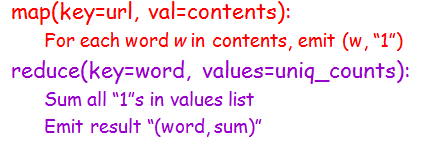
\includegraphics[height=60pt]{keyan/map1.png}
    \end{center}
    \end{block}

    \begin{block}{Count, Illustrated}
    \begin{center}
    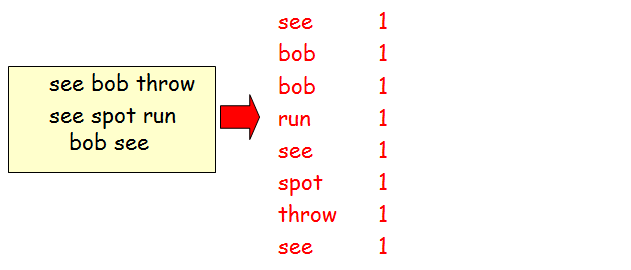
\includegraphics[height=80pt]{keyan/map2-1.png}
    \end{center}
    \end{block}
\end{frame}

\begin{frame}[c]{Count Words in Docs}
    \begin{block}{Algorithm Code Demo}
    \begin{center}
    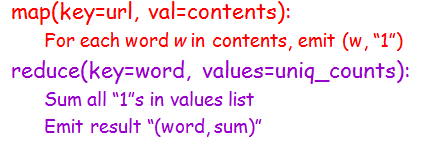
\includegraphics[height=60pt]{keyan/map1.png}
    \end{center}
    \end{block}

    \begin{block}{Count, Illustrated}
    \begin{center}
    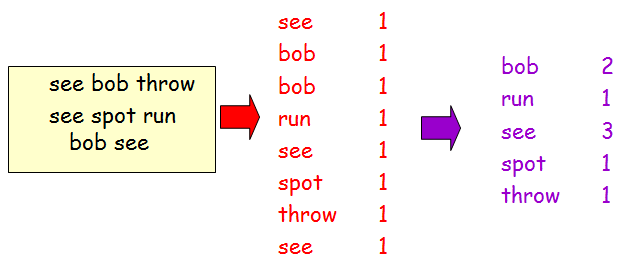
\includegraphics[height=80pt]{keyan/map2-2.png}
    \end{center}
    \end{block}
\end{frame}
%-- illustrator --
\begin{frame}{More Demos}
\begin{itemize}
    \item 倒转网络连接图
        \begin{itemize}
        \item Map在网页(source)中搜索链接目标(target),输出为(target, source)
        \item Reduce合并相同的target,输出(target, list(source))
        \end{itemize}
    \item 计算URL访问频率
        \begin{itemize}
        \item Map处理日志中web页面请求的记录,输出(URL, 1)
        \item Reduce把相同URL的value累加,产生(URL,记录总数)结果
        \end{itemize}
\end{itemize}
\end{frame}

\subsection{框架实现}
\begin{frame}{结构}
    \begin{block}{模型实现} \begin{center}
    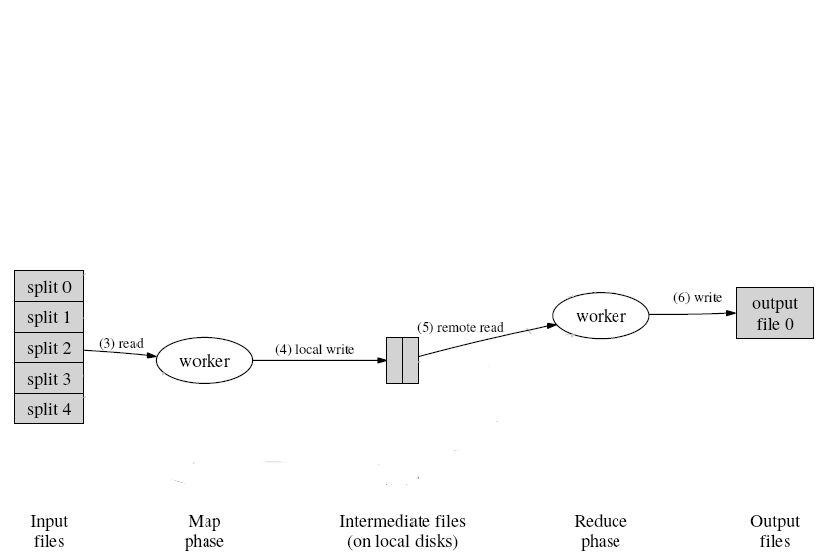
\includegraphics[height=180pt]{keyan/mapreduce.png}\\
    \end{center}\end{block}
\end{frame}

\begin{frame}{结构}
    \begin{block}{更多的worker加入} \begin{center}
    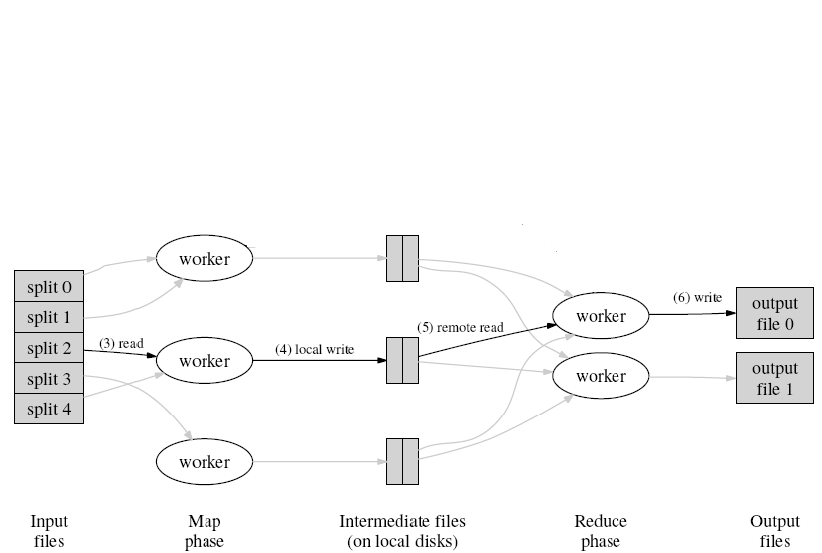
\includegraphics[height=180pt]{keyan/mapreduce1.png}\\
    \end{center}\end{block}
\end{frame}

\begin{frame}{结构}
    \begin{block}{中央控制master} \begin{center}
    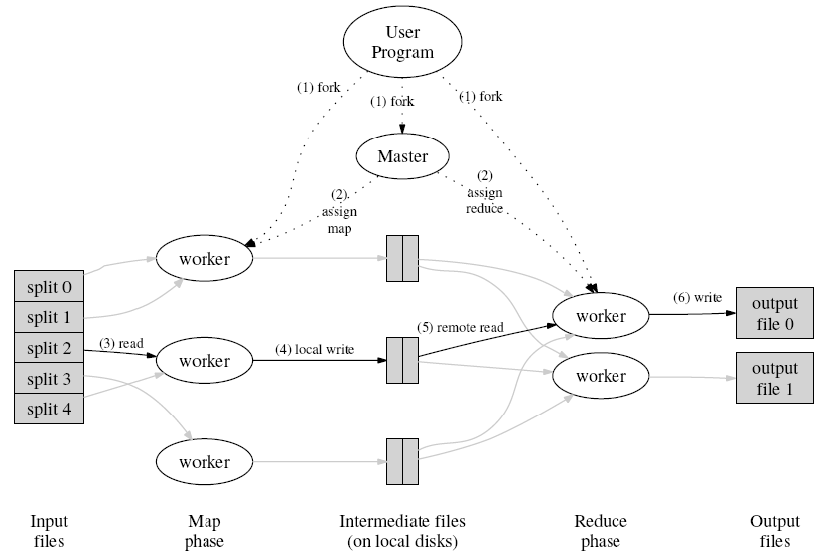
\includegraphics[height=180pt]{keyan/mapreduce2.png}\\
    \end{center}\end{block}
\end{frame}

\subsection{容错}
%--worker出错--
\begin{frame}{容错}
    \begin{block}{worker故障}
    \begin{center} 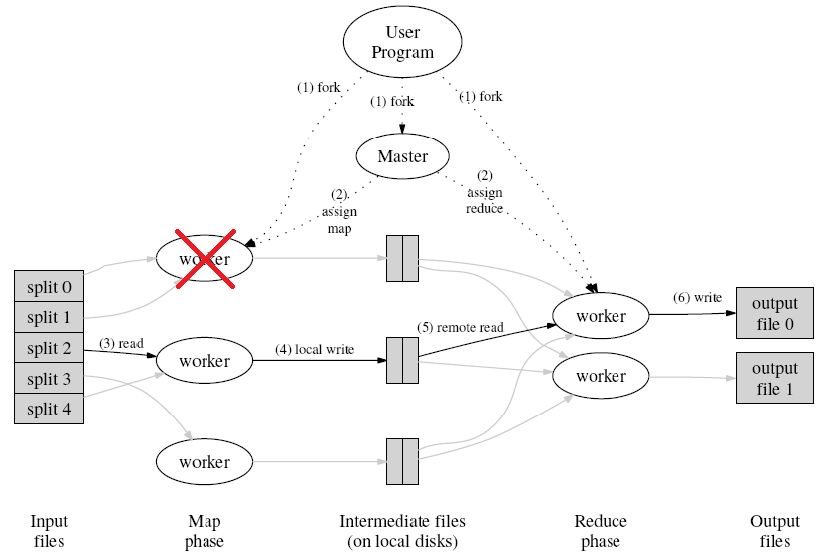
\includegraphics[height=180pt]{keyan/mapreduce_worker_wrong.png} \end{center}
    \end{block}
\end{frame}
\begin{frame}{容错}
    \begin{block}{worker故障}
    \begin{center} 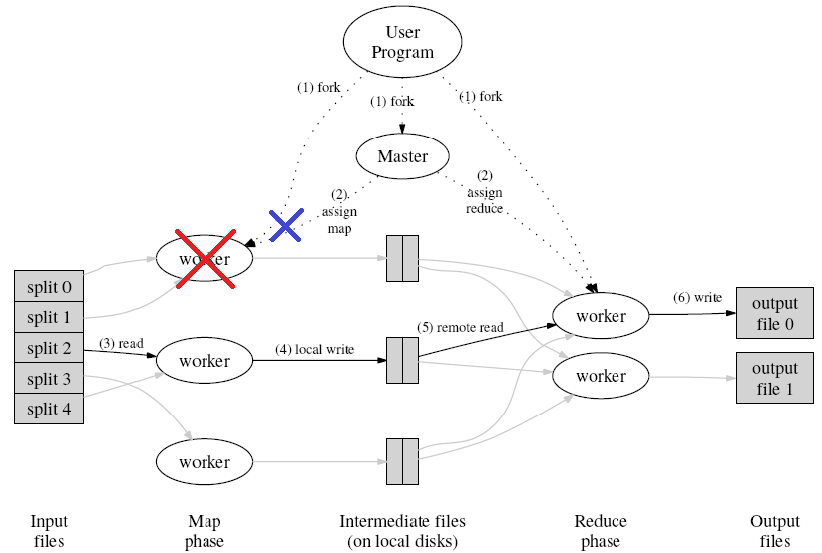
\includegraphics[height=180pt]{keyan/mapreduce_worker_wrong1.png} \end{center}
    \end{block}
\end{frame}
\begin{frame}{容错}
    \begin{block}{worker故障}
    \begin{center} 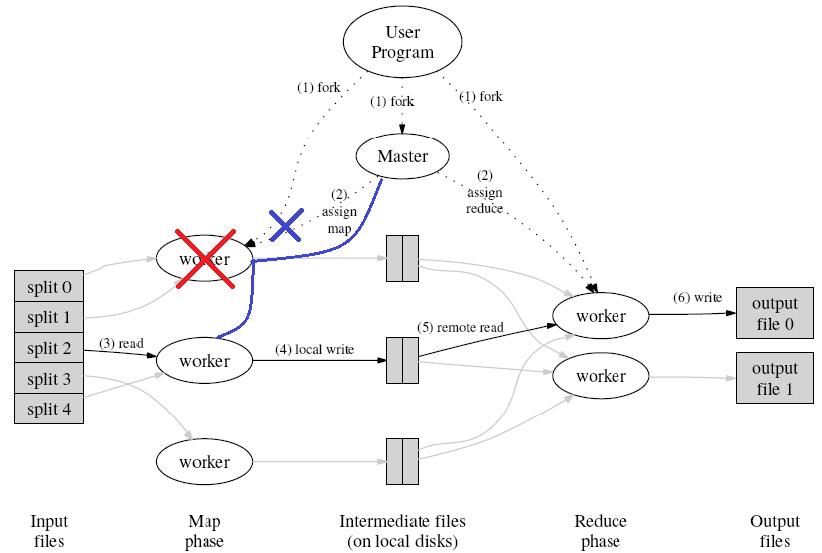
\includegraphics[height=180pt]{keyan/mapreduce_worker_wrong2.png} \end{center}
    \end{block}
\end{frame}
%--master出错--
\begin{frame}{master失败}
    \begin{block}{master故障}
    \begin{center} 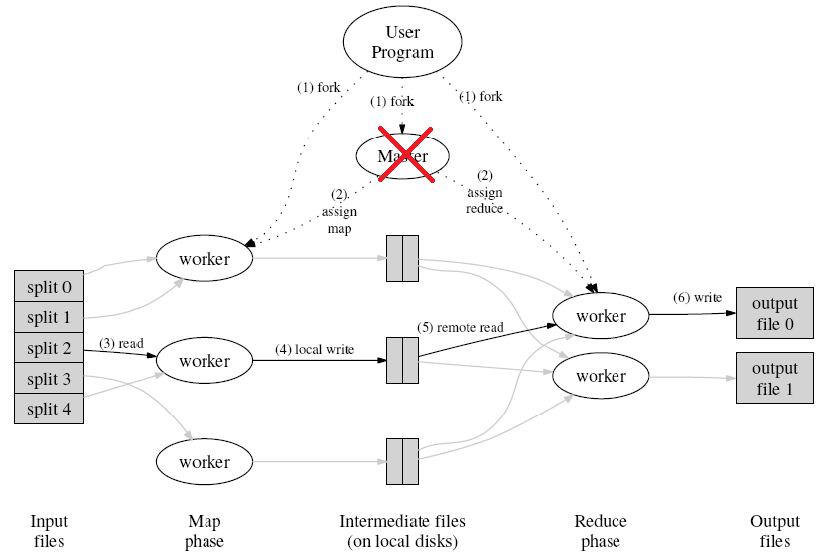
\includegraphics[height=180pt]{keyan/mapreduce_master_wrong.png} \end{center}
    \end{block}
\end{frame}
\begin{frame}{master失败}
    \begin{block}{根据最后断点,重新建立进程}
    \begin{center} 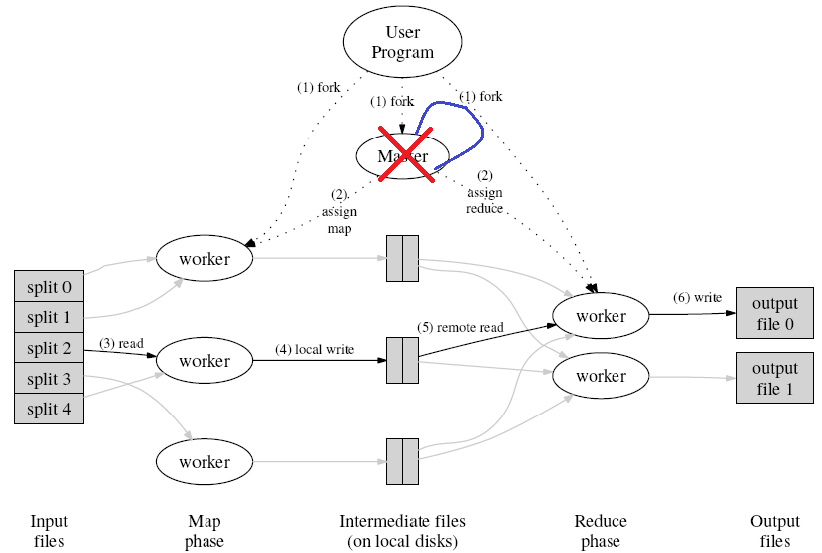
\includegraphics[height=180pt]{keyan/mapreduce_master_wrong2.png} \end{center}
    \end{block}
\end{frame}

\begin{frame}{性能}
\begin{itemize}
    \item 在2000台机器上运行
    \item 使用$2\times 10^5$个map任务 \& 5000个reduce任务
\end{itemize} 
\centerline{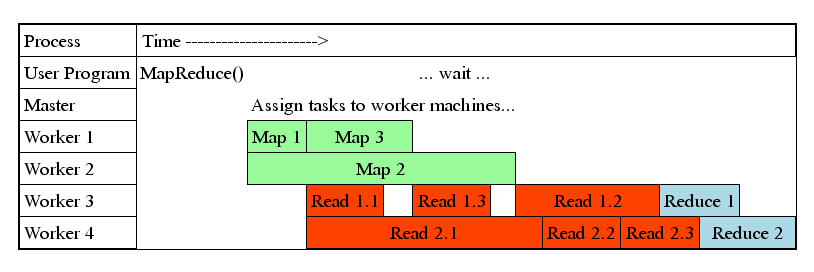
\includegraphics[height=80pt]{keyan/pp.png} }
\end{frame}

\begin{frame}{性能}
\begin{overprint}
    \onslide<1>\centerline{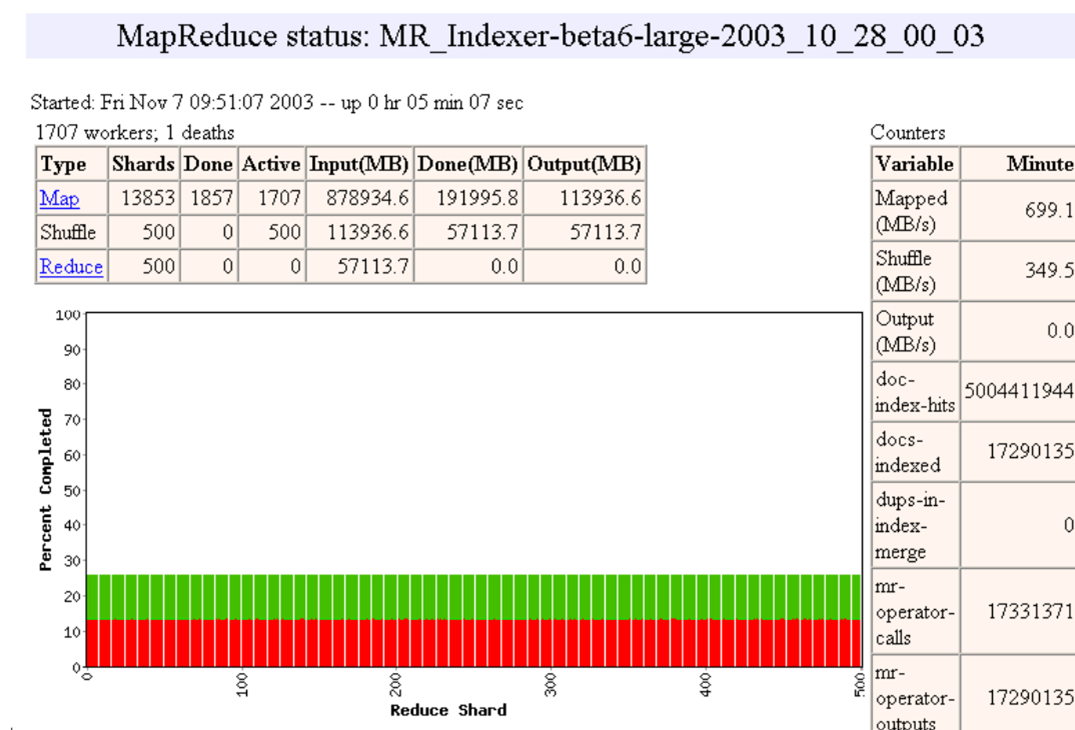
\includegraphics[height=180pt]{keyan/p1.png} }
    \onslide<2>\centerline{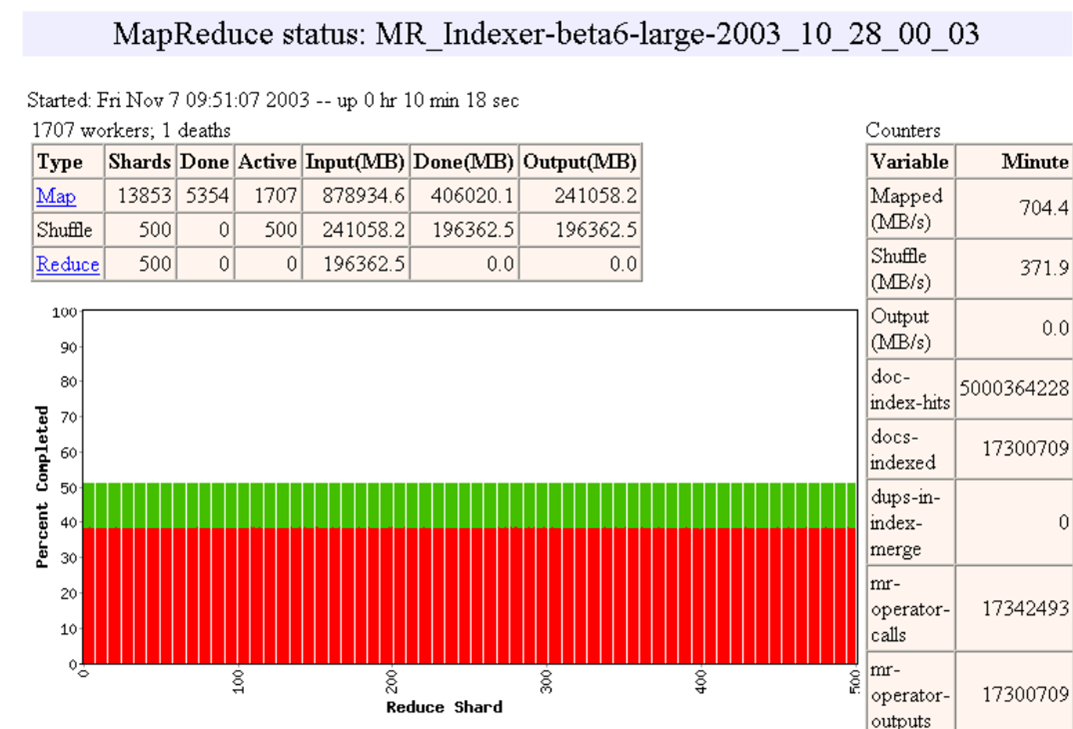
\includegraphics[height=180pt]{keyan/p2.png} }
    \onslide<3>\centerline{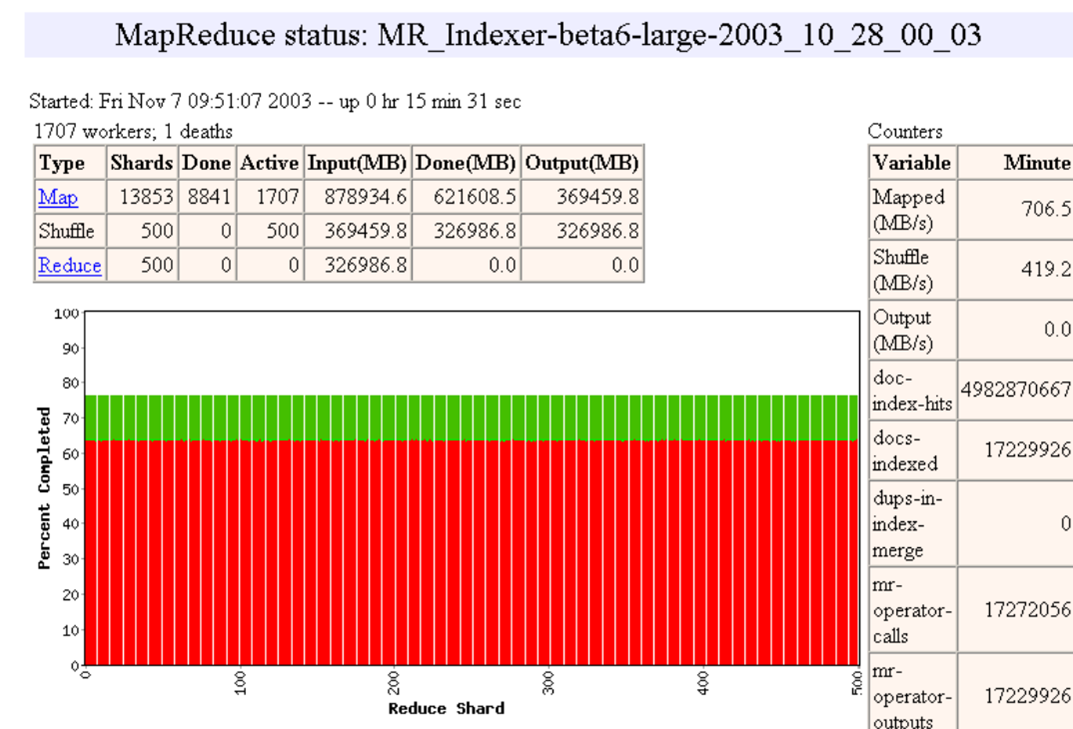
\includegraphics[height=180pt]{keyan/p3.png} }
    \onslide<4>\centerline{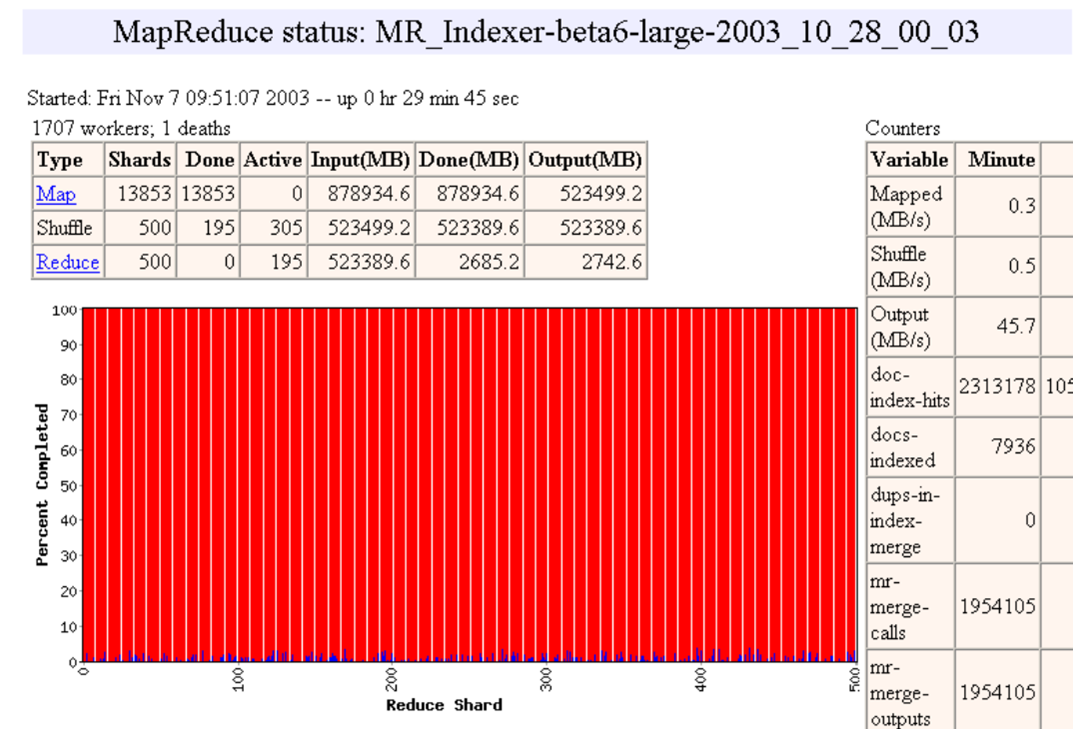
\includegraphics[height=180pt]{keyan/p4.png} }
    \onslide<5>\centerline{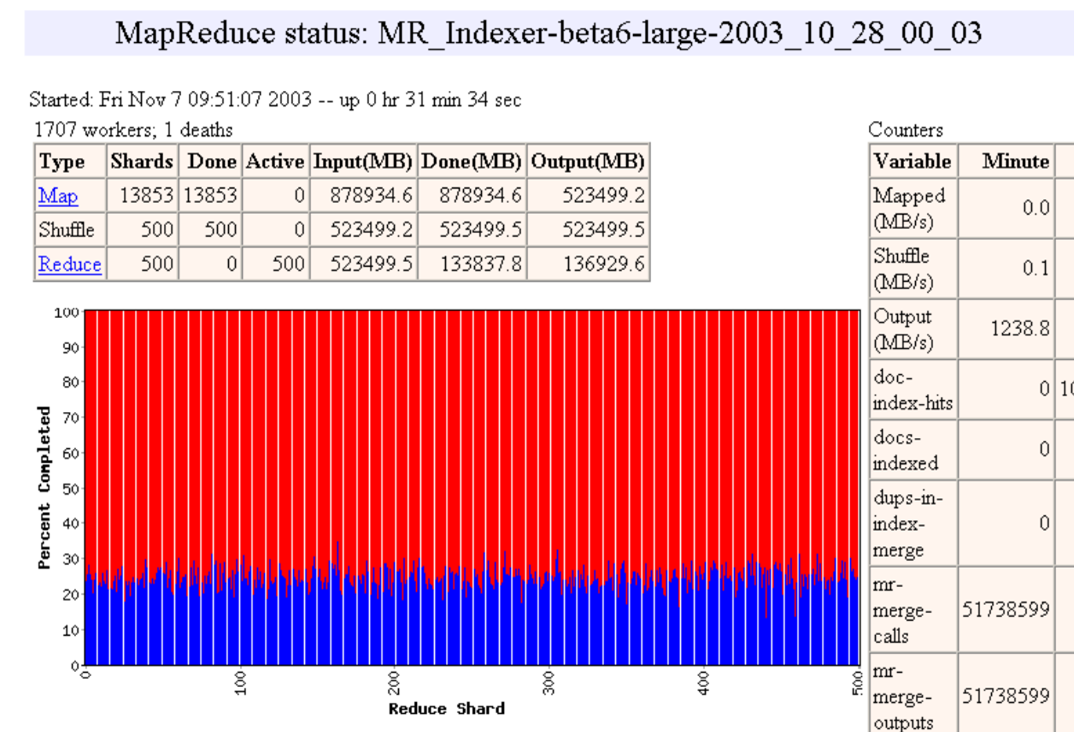
\includegraphics[height=180pt]{keyan/p5.png} }
    \onslide<6>\centerline{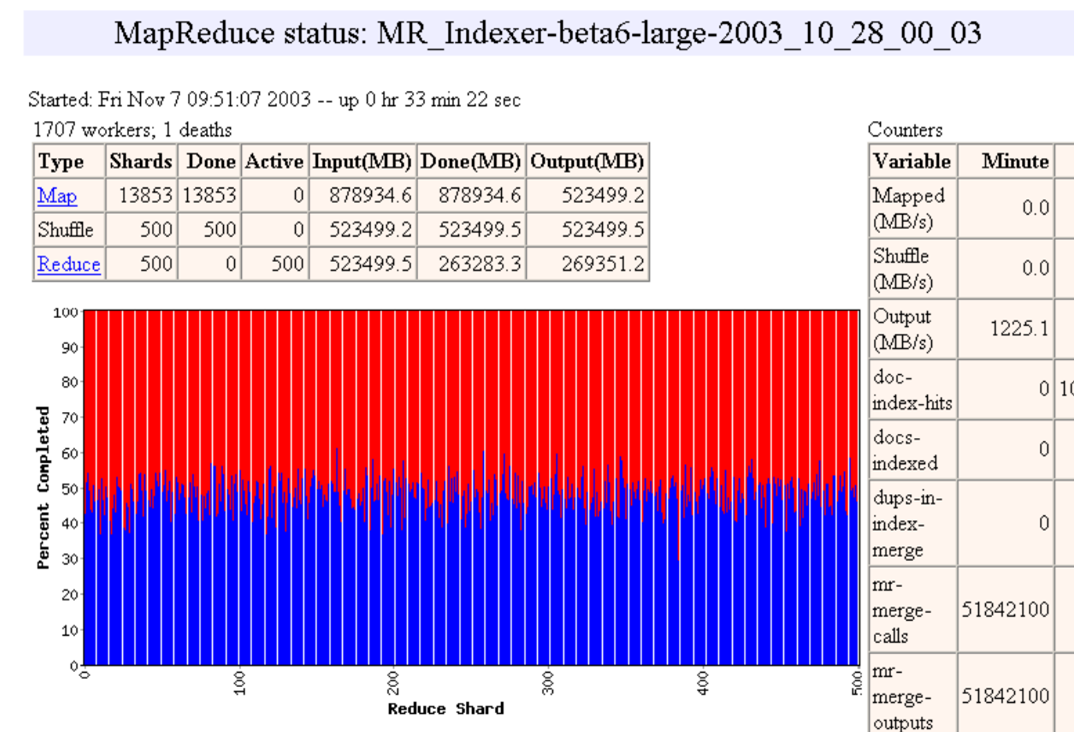
\includegraphics[height=180pt]{keyan/p6.png} }
    \onslide<7>\centerline{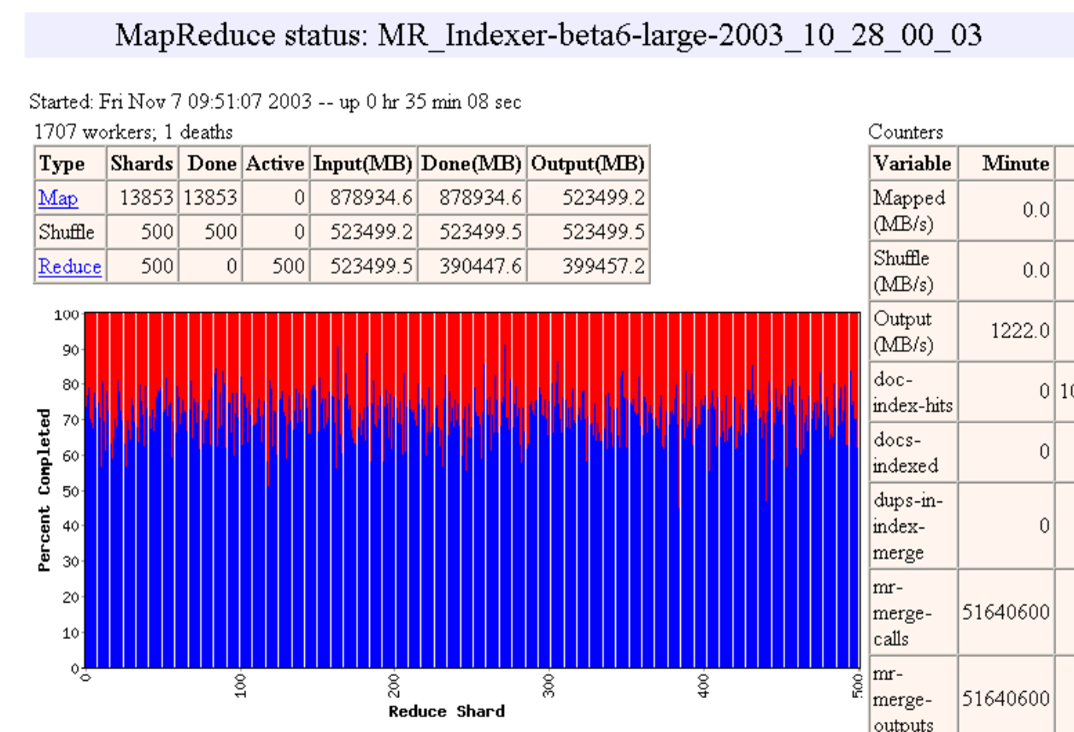
\includegraphics[height=180pt]{keyan/p7.png} }
    \onslide<8>\centerline{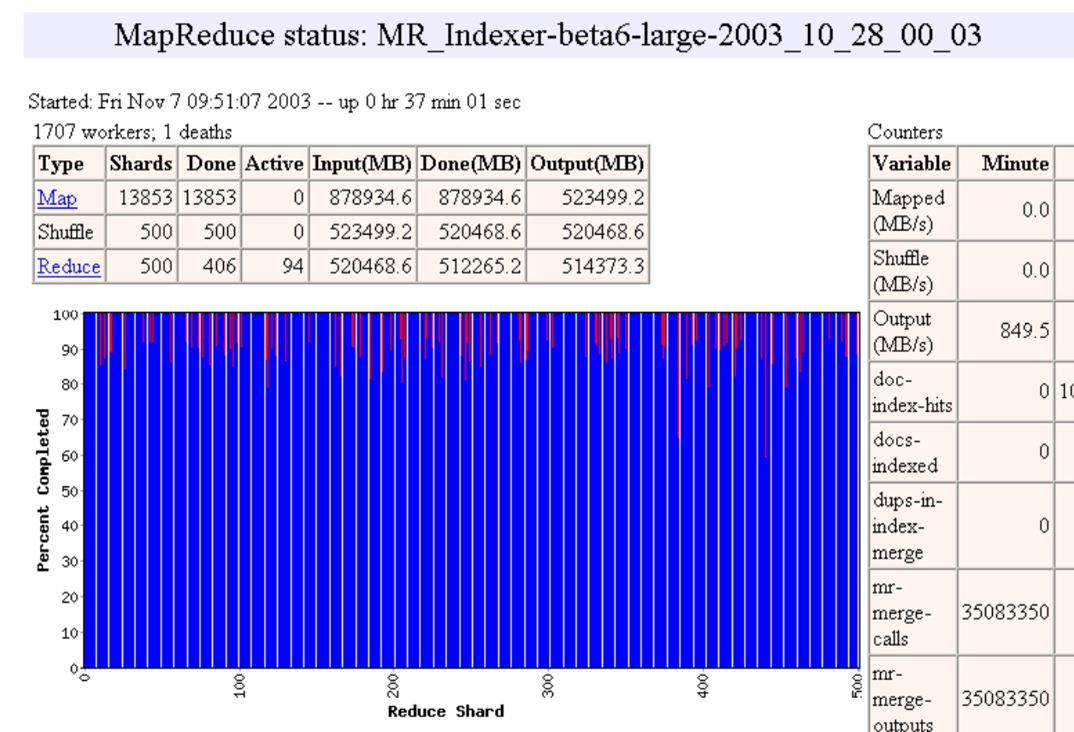
\includegraphics[height=180pt]{keyan/p8.png} }
    \onslide<9>\centerline{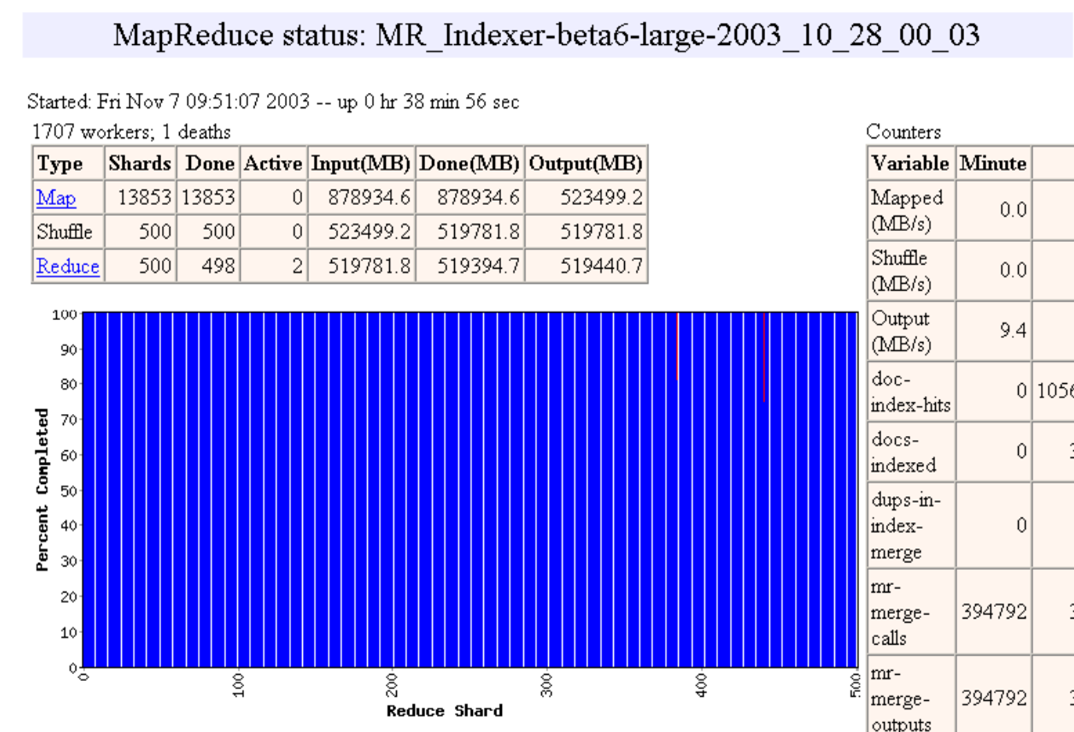
\includegraphics[height=180pt]{keyan/p9.png} }
    \onslide<10>\centerline{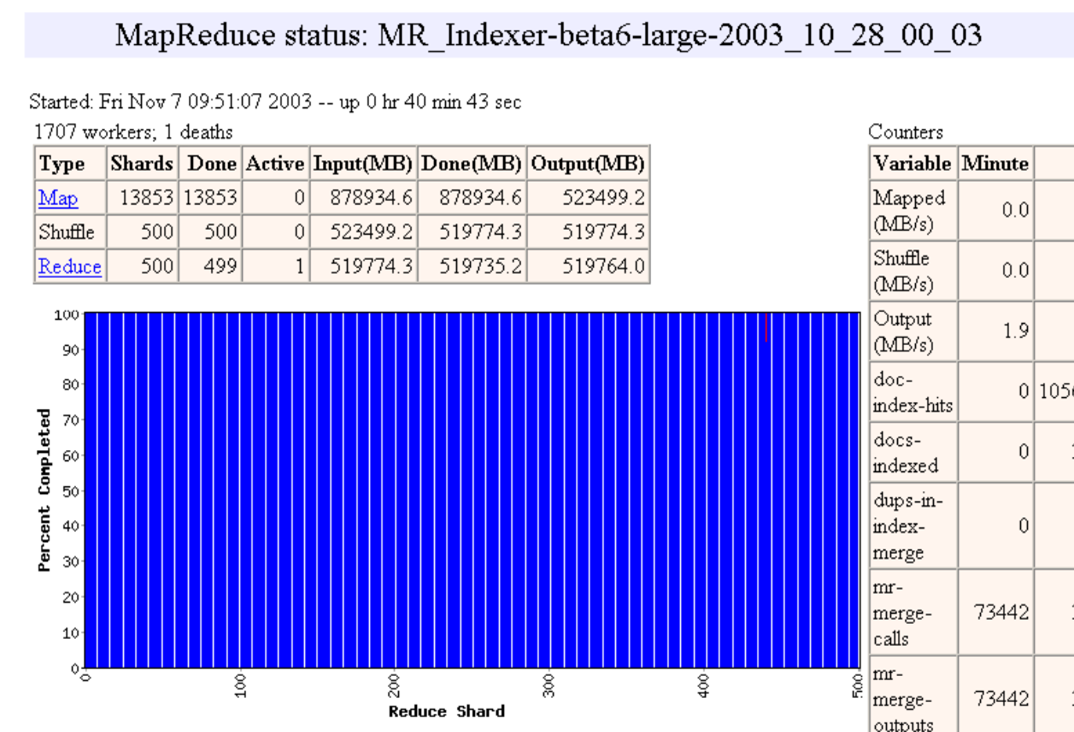
\includegraphics[height=180pt]{keyan/p10.png} }
\end{overprint}
\end{frame}




\begin{frame}{References}

\begin{thebibliography}{10}
\bibitem{mapreduce} [Jeffrey Dean and Sanjay Ghemawat, 2004]
    \newblock Google,Inc
    \newblock \emph{MapReduce:Simplified Data Processing on Large Cluster}, 2004
\bibitem{mapclass} [Dan Weld]
    \newblock \emph{Dan Weld's class at U. Wanshington}
\bibitem{mapreduceonline} [Rajesh Gadipuuri]
    \newblock \emph{MapReduce Online}
\bibitem{m}[Anand Rajaraman, Dan Weld]
    \newblock Stanford Univ. , Univ. of Washington
    \newblock \emph{Map Reduce Architecture}
\end{thebibliography}
\end{frame}

\begin{frame}{Conclusion}
\begin{itemize}
    \item Map/Reduce良好的模型抽象
    \item 极大地简化了大规模计算
    \item 弹性容错\&可靠的计算框架
    \item 数量取胜,有效而廉价
\end{itemize}
\end{frame}

\end{document}
